\documentclass{standalone}
\usepackage{tikz}
\begin{document}
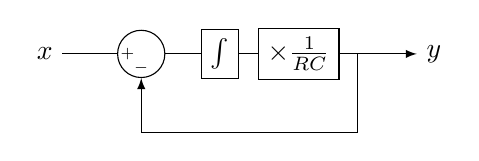
\begin{tikzpicture}
  \node[draw,fill=white,circle,minimum size=.6cm, inner sep=1pt] (p) {};
  \node[anchor=south, inner sep=1.5pt] at (p.south) {\tiny$-$};
  \node[anchor=west, inner sep=1pt] at (p.west) {\tiny$+$}; 
  \draw[-latex] (p) to[latex-] ++(-1,0) node[anchor=east] {$x$}
  (p) to[-latex]
  ++(1,0) node[draw,fill=white] {$\int$}
  --++(1,0) node[draw,fill=white] {$\times\frac{1}{RC}$} 
  --++(.75,0) coordinate (q) to[-latex]
  ++(.75,0) node[anchor=west] {$y$};
  \draw[-latex] (q) to ++(0,-1) -| (p.south);
\end{tikzpicture}
\end{document}

%%% Local Variables:
%%% mode: latex
%%% TeX-master: "../date2018"
%%% End:
